\chapter{Implementation and Results}

% ---GRAPHS TO PRODUCE---
%
% >SIMULATION<
% slidingMode_theta
% slidingMode_x
% slidingMode_u
%
% swingAndCatch_theta
% swingAndCatch_x
% swingAndCatch_u
%
% >TEST<
% slidingMode_test_theta
% slidingMode_test_x
% slidingMode_test_u
%
% swingUp_test_theta
% swingUp_test_x
% swingUp_test_Edelta
% swingUp_test_u
%
% swingAndCatch_test_theta
% swingAndCatch_test_x
% swingAndCatch_test_u

\fxnote{Write about FIR filter for swing-up}

\begin{figure}[H]
  \hspace{-10pt}
  \captionbox
  {
    Test of sliding mode controller starting at zero. The controller is subjected to a disturbance after which it rebalances successfully bringing the angle back to zero.
    \label{fig:slidingMode_test_theta}
  }
  {
    \hspace{-1cm}
    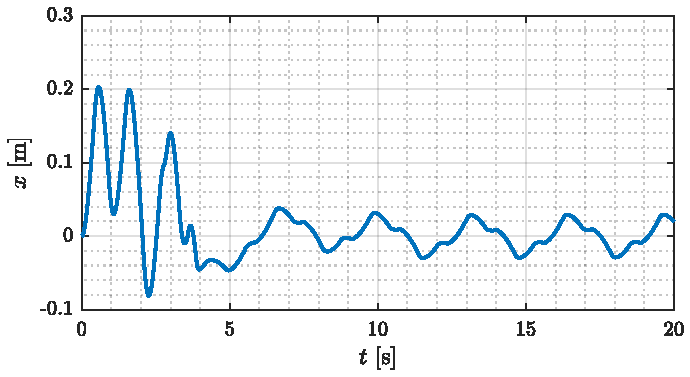
\includegraphics[width=.4\textwidth]{figures/x_4_conX}
  }
  \hspace{20pt}
  \captionbox 
  {
    The cart returns to zero once the pendulum is rebalanced.
    \label{fig:slidingMode_test_x}
  }
  {
    \hspace{-1cm}
    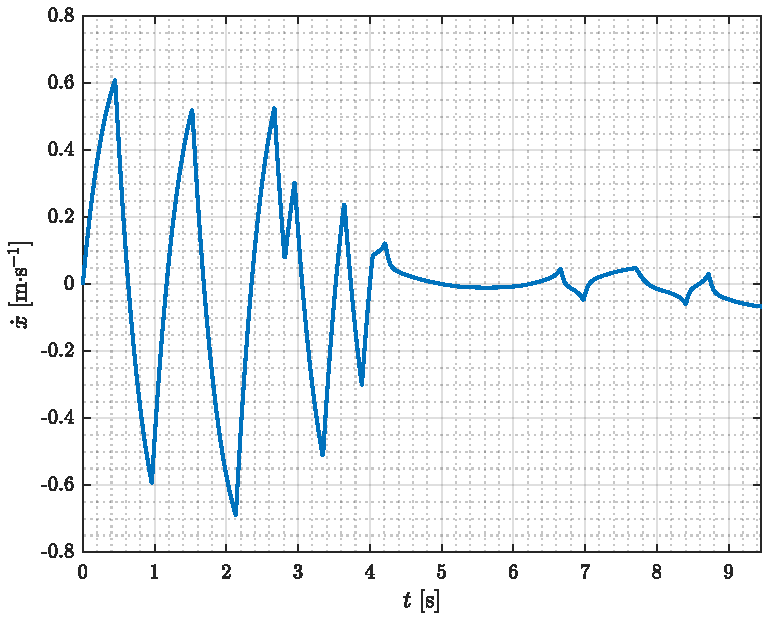
\includegraphics[width=.4\textwidth]{figures/xDot_4_conX}
  }  
\end{figure}

\begin{figure}[H]
  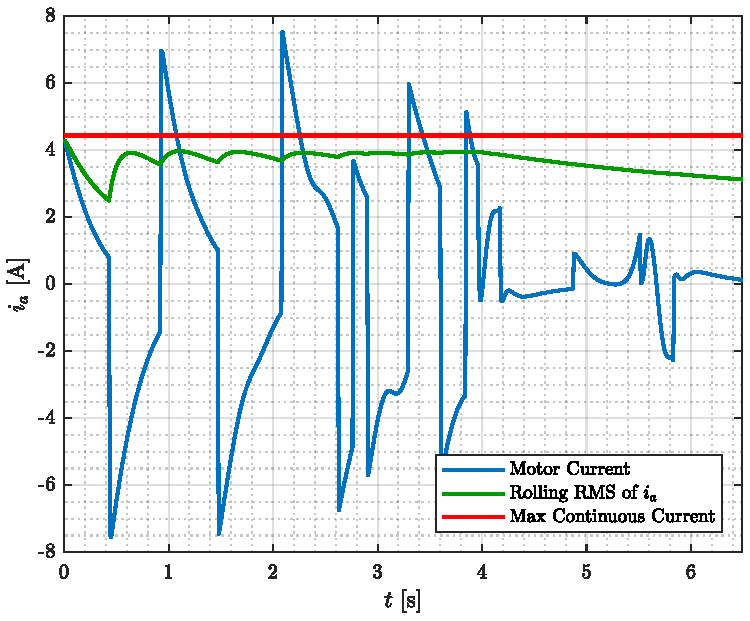
\includegraphics[width=.42\textwidth]{figures/ia_4_conX}
  \caption{ u  }
  \label{fig:slidingMode_test_u}
\end{figure}

\begin{figure}[H]
  \hspace{-10pt}
  \captionbox
  {
    The swing-up controller approaches the equilibrium and eventually reaches the heteroclinic orbit.
    \label{fig:swingUp_test_theta}
  }
  {
    \hspace{-1cm}
    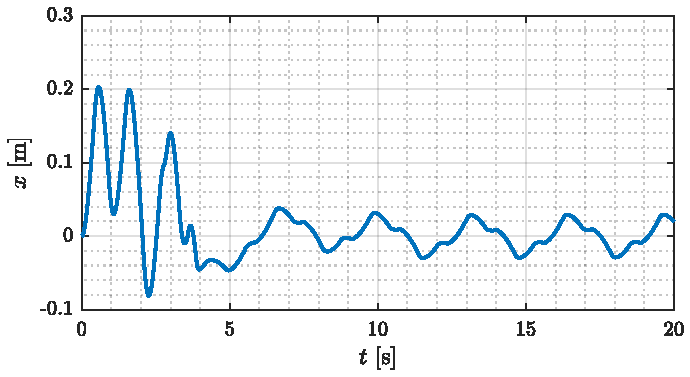
\includegraphics[width=.4\textwidth]{figures/x_4_conX}
  }
  \hspace{20pt}
  \captionbox 
  {
    Once the energy reference is tracked, the cart maintains a closer proximity to zero on the rail.
    \label{fig:swingUp_test_x}
  }
  {
    \hspace{-1cm}
    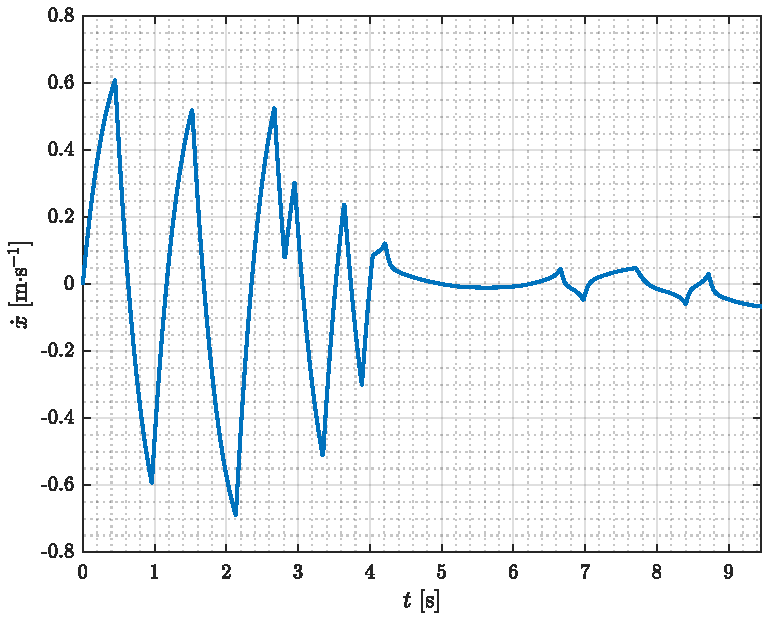
\includegraphics[width=.4\textwidth]{figures/xDot_4_conX}
  }  
\end{figure}

\begin{figure}[H]
  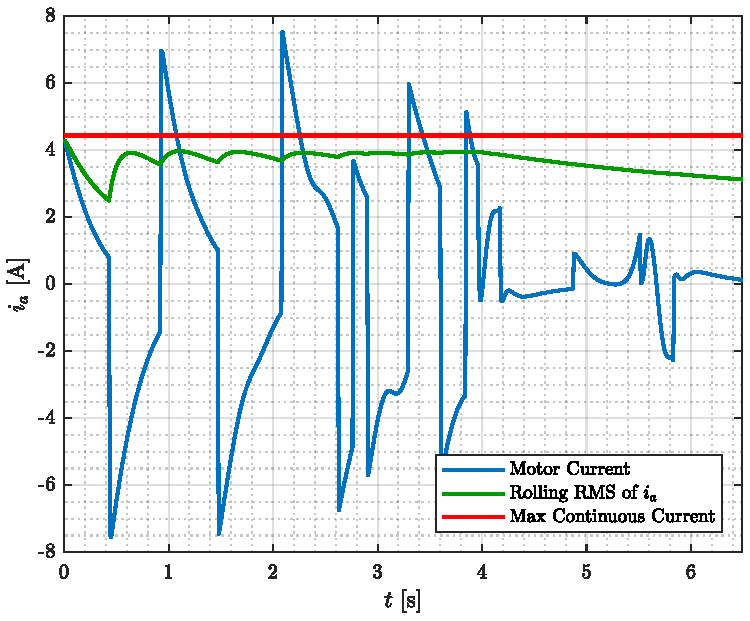
\includegraphics[width=.42\textwidth]{figures/ia_4_conX}
  \caption{From the test in \autoref{fig:swingUp_test_theta} and \ref{fig:swingUp_test_x} energy reference is reached.}
  \label{fig:swingUp_test_Edelta}
\end{figure}

\begin{figure}[H]
  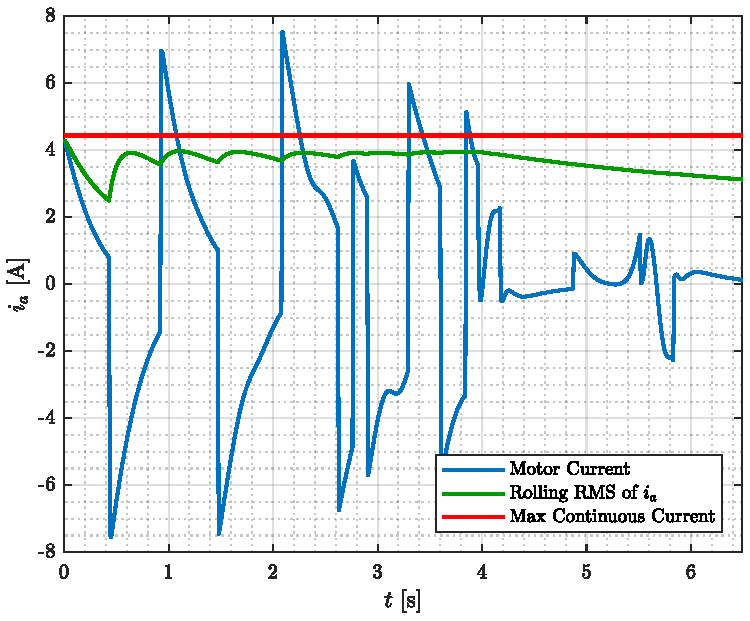
\includegraphics[width=.42\textwidth]{figures/ia_4_conX}
  \caption{ u  }
  \label{fig:swingUp_test_u}
\end{figure}

Though the swing-up controller reaches the heteroclinic orbit, it takes some time to get there. It is possible to approach the equilibrium faster by adding some energy to the energy reference. This will mean that the swing-up controller would eventually cause some entry velocity at equilibrium and overshoot. However, since the catch controller is enabled close to equilibrium, this adjustment causes catch after fewer swings. Further, the sliding mode controller is helped by some entry velocity at the maximum catch angle.\fxnote{note the adjustment, Edelta eq Edelta plu addedE}

\begin{figure}[H]
  \hspace{-10pt}
  \captionbox
  {
    Test of the final design of swing-up with the higher energy reference and sliding mode controller successfully catching the pendulum after 7 swings.
    \label{fig:swingAndCatch_test_theta}
  }
  {
    \hspace{-1cm}
    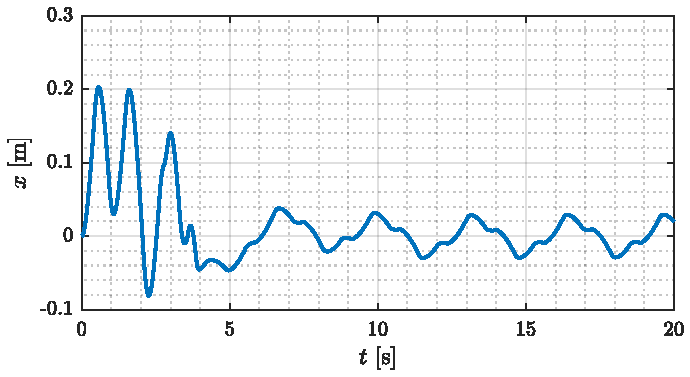
\includegraphics[width=.4\textwidth]{figures/x_4_conX}
  }
  \hspace{20pt}
  \captionbox 
  {
    The cart keeps around zero on the rail, especially after the pendulum angle is controlled to zero.
    \label{fig:swingAndCatch_test_x}
  }
  {
    \hspace{-1cm}
    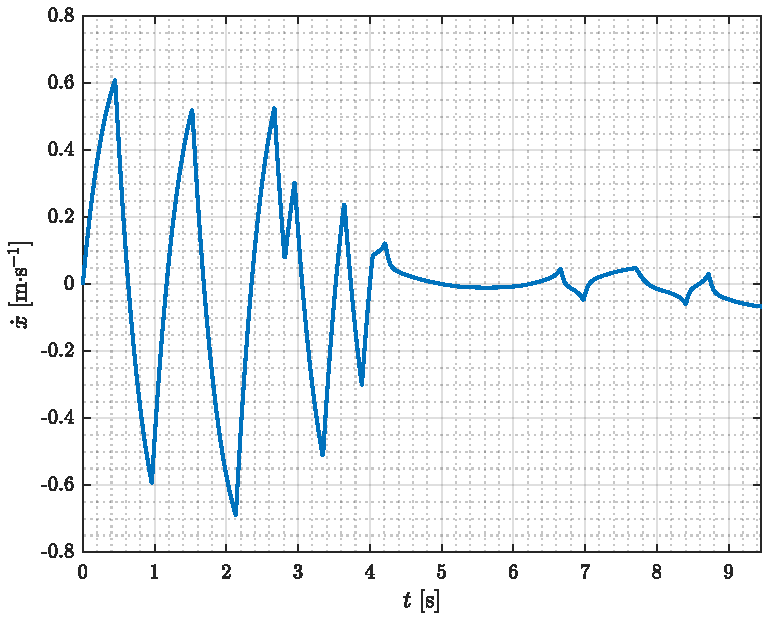
\includegraphics[width=.4\textwidth]{figures/xDot_4_conX}
  }  
\end{figure}

\begin{figure}[H]
  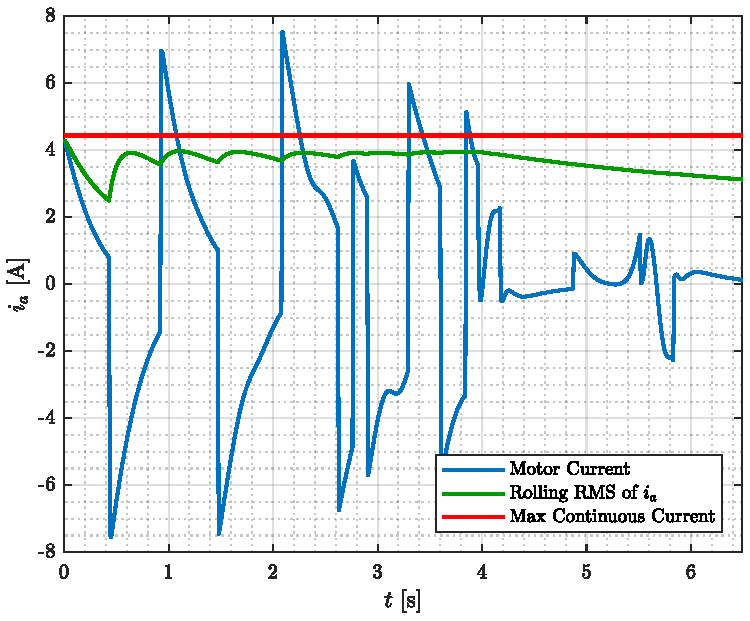
\includegraphics[width=.42\textwidth]{figures/ia_4_conX}
  \caption{ u  }
  \label{fig:swingAndCatch_test_u}
\end{figure}

In the implementation, the angle is wrapped around using modulo such that zero is always found at the upright position. This means catch can happen from either side of the swing and even after overshoot. Wrapping the angle in this way causes a discontinuity at $\pm \pi$ at the stable equilibrium. This however does not cause a problem for the swing up sequence, but both the wrapped angle and the continuous are kept accessible, allowing the Kalman filter\fxnote{Kalman} to use the continuous version.